\chapter{State of the Art} \label{chap:sota}

\section*{}

This chapter starts with an overview of online marketing in the last few years, followed by a review of
what was done and is been done in the field of predicting the traffic of a network.
Lastly, it is done a review of data mining algorithms that can be used to solve the same kind of problems as this thesis.

\section{Online Advertising Overview}

Before entering in details about the state of the art of the technologies that can be used to
help solve the presented problem, it is better to explain some basic concepts about the world of online advertising.

All advertising has the main purpose of getting a message to the people that will impact or influence them in some way,
therefore the same goal is applied to online advertising.
One of the metrics of advertising are impressions, which correspond to the number of times a user sees the message (the ad).\cite{kOA}
\textbf{Ads} can present itself in various sizes\cite{kOA2}, forms and locations \cite{kOA3}, and these characteristics are chosen both by the advertiser
and the publisher to better serve their purpose.
\textbf{Campaigns} are composed by two big parts, which are the ads that compose it and the target population that they pretend to reach,
including the rules of this targeting. For example, \textbf{frequency capping} to limit the number of times the same advertising is shown to the user \cite{kOA},
avoiding, in this way, showing the same ad multiple times in a row to the same user, that can lead to a bad response from his part.\cite{Buchbinder20141}

Nowadays, the main pricing models of online advertising are:
\begin{itemize}
\item\textbf{Cost-per-Mile} where the advertiser pays per impression. The main problem of this model is the advertiser as to pay to the publisher even
if the ad doesn't lead to any profit.
\item\textbf{Cost-per-Click} where the advertiser pays per click to the publisher. This model is more expensive per unit\cite{Performics}, but on overall can be more
profitable\cite{Performics} if the audience of the websites where the ad is imprinted is more interested in that kind of product/service\cite{Andrea2004}.
\item\textbf{Cost-per-lead} where the advertiser pays for a lead. If this model is being used the advertiser doesn't pay per number of impressions nor per clicks. Instead, pays only
if he gets valid information about the user, like the information of a sign up form for a community.
\item\textbf{Cost-per-Action} or \textbf{Cost-per-Order} where the advertiser is charged per buy or action. This model is similar to CPL but has in mind an instantaneous return of
the investment.
\end{itemize}

Traditionally, publishers sell their space to advertisers in bulk (\textbf{Ad networks}) this method has its \textit{ups} and \textit{downs}.
The obvious \textit{up} is that sometimes the advertiser gets premium spots at low prices.
On the other hand, one of the biggest drawbacks is that when the advertiser buys the impressions as a
closed package, sometimes impressions are not maximized in terms of profit.
Other problem of traditional methods that, although the \emph{CPA} and \emph{CPL} pricing methods minimize the risk for the advertiser, the responsibility of
optimizing conversion rate\footnote{ See, e.g., \url{http://www.marketingterms.com/dictionary/conversion_rate/}} is still
on the ad network hands.\cite{Yuan:2013:RBO:2501040.2501980}

In the past few years, a new model called \textbf{Real Time Bidding}\index{Real Time Bidding}\index{RTB} has been gaining terrain \cite{Adfonic}.
\emph{RTB}, as the name gives, is a market where publishers offer his advertisement space and advertisers bid over it in real time. This allow publishers to get
the best value for their space and advertisers get the best placement for their advertisement.

There are three main players in the world of \emph{RTB}\index{Real Time Bidding}:
\begin{itemize}
\item The \textbf{Demand Side Platform}\index{DSP} is a tool used by the advertisers to act on their behalf on the \emph{RTB}. \emph{DSPs}\index{DSP} allows them to set
their campaigns' parameters and to monitor the performance of the campaign. This way the advertisers try to get the best performance of their campaigns because 
\emph{DSPs} use algorithms driven by performance data.\cite{Gern201230}
\item The \textbf{Publisher} provides the inventory, that is comprised by accesses made by users. In some cases, the publisher uses \textbf{Supply Side Platforms}.
\emph{SSPs} help the publisher to better manage his inventory, and even let him set a reserve price for their inventory.\cite{Yuan:2013:RBO:2501040.2501980}
\item The \textbf{Ad Exchange} looks a little like a stock exchange, but in reality is a software platform that mediates the exchange. This exchange takes place in
a few milliseconds while the page loads.
\end{itemize}

\emph{RTB} allows some features of paid search advertising everywhere \cite{Gern201230}, because it allows the advertiser to better select
the inventory\footnote{ this inventory is made of user accesses} where he wants their campaigns to run on.
The flexibility that \emph{RTB} gives to all the intervinients of this exchange is what demands the necessity of predicting the future inventory, to
better access its value.


\section{Network Traffic Prediction}\label{sec:network}

\section{Data Mining}\label{sec:datamining}
%\begin{quote}
''Data mining is about solving problems by analyzing data already present in databases.''\cite[p. 5]{Witten:2005:DMP:1205860}
%\end{quote}
. Furthermore, consists in a vast number of techniques used to find interesting patterns in large datasets and translate
that huge quantity of raw data in information and/or knowledge. 

Data mining uses techniques from various fields, mostly from mathematics and computer science,
such as artificial intelligence, machine learning and statistics.
Data mining is sometimes referred as the natural evolution of information technologies \cite[p. 1]{HanKam06}

There are lots of methods of data mining, which can be separated in two groups: descriptive data mining and predictive
data mining \cite{Fayyad96knowledgediscovery}.
The main focus of the first group is to find the underlying structure of a given dataset, which methods try to find relationships and connections
between the values, without have the goal of predicting the future. On the other hand,
predictive data mining goal is to predict explicit values from patterns found on the original data set. These methods are used to build models based on past
events that can be used to predict future events.
This division is not always sharp and in some cases an algorithm mixes the two methods (predictive \& descriptive)\cite{Fayyad96knowledgediscovery}.

According to previous statements it is easy to notice that data mining doesn't apply only to one set of problems and can be used to solve many different types of
problems. The most common methods are:
\begin{itemize}
\item \textbf{Anomaly Detection} tries to discover abnormal data on the dataset. This can be useful for identifying suspicious activity on a bank
account log for example.
\item \textbf{Classification} is a method to identify which of a given set of categories a new observation belongs.
\item \textbf{Clustering} is the method of grouping similar data together, in a finite number of categories, without prior knowledge of
the characteristics of each group or the data.
\item \textbf{Dependency modeling} tries to find associations between variables. For example, trying to find out which clothes go well together.
\item \textbf{Summarization} is a method to provide an overview of the dataset, sometimes including visual representation and/or report generation.
\item \textbf{Regression} tries to find a function that can represent a given dataset with the least error associated.
\end{itemize}

\subsection{Classification Algorithms}\label{sec:classification}

\subsubsection{Decision Trees}

Decision trees algorithms use a decision tree as a predictive model where all internal nodes (non-leaf nodes) are a test for the value of an attribute that will
ultimately lead to a leaf node with the class attribute value (see example in figure~\ref{fig:dtree}).
In other words, the selection of the class value is only based on the attribute values of the entry.\cite{HanKam06}

\begin{figure}[h]
  \begin{center}
    \leavevmode
    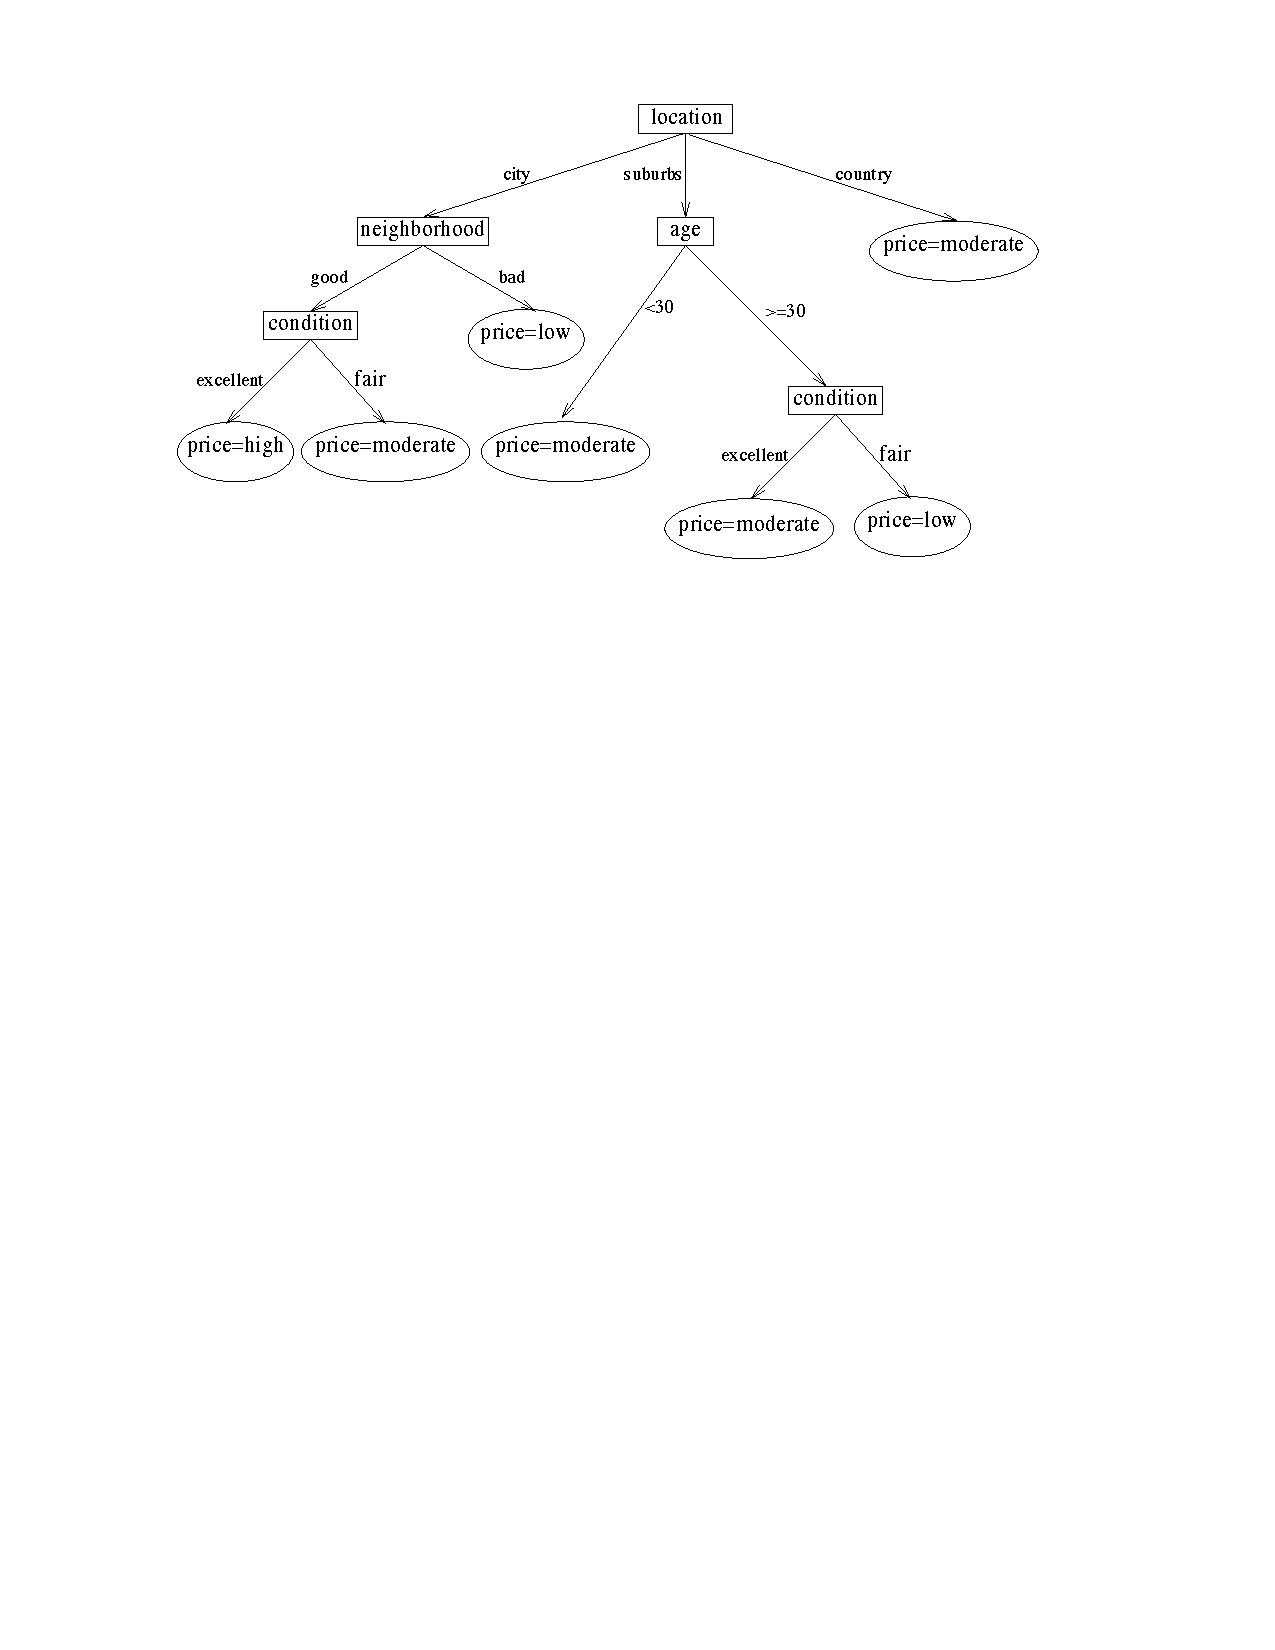
\includegraphics[width=0.86\textwidth]{dt}
    \caption{Example of a decision tree, Rectangles represent internal nodes and ovals represent leaf nodes (possible solution)\cite{KER:70953}}
    \label{fig:dtree}
  \end{center}
\end{figure}


\subsubsection{Random Forests}

\subsubsection{Support Vector Machines}

\subsubsection{KNN}

\subsection{Clustering Algorithms}\label{sec:clust}

\subsection{Regression Algorithms}\label{sec:regr}

\subsection{Instance-based regression algorithms}\label{sec:instance}

\subsection{Time Series Analysis}\label{sec:timeseries}
